\documentclass[aspectratio=169]{beamer}
\usetheme{metropolis} 
% \usetheme[progressbar=frametitle]{metropolis}
\usepackage{appendixnumberbeamer}
 
\usepackage{booktabs}
\usepackage[scale=2]{ccicons}

\usepackage{xspace}
\newcommand{\themename}{\textbf{\textsc{metropolis}}\xspace}

\usepackage[backend=biber,doi=true, natbib=true,style=ieee ]{biblatex}
\addbibresource{main.bib}

\title{Earth at night}
\subtitle{The visualisation of average radiance in 3 areas}
\date{\today}
% \date{}
\author{Zhen Chen (John), Huajie Xu, Shengzhu Wang, Wenjie Tong, SiXiang Xiong}
% \institute{A2 Inc}
\titlegraphic{\hfill
\includegraphics[height=1.5cm]{images/logo.png}}

\begin{document} 
\maketitle

\begin{frame}{}
  \setbeamertemplate{section in toc}[sections numbered]
  \tableofcontents[hideallsubsections]
\end{frame}

\section{Introduction to background}

\begin{frame}[fragile]{Background: World Bank Nightime Light Data}

  \begin{columns}
    \column{0.5\textwidth}
    World Bank Nightime Light Data consists of a lot of satellite imagery 
    stored in Amazon Web Services (AWS) (Fig.~\ref{wbs3}). 
    
    Latest files from 2012 to 2020 are generated by the sensor 
    named Visible Infrared Imaging Radiometer Suite Day-Night Band (VIIRS DNB) \citep{WorldBan13:online}.
    
    \column{0.5\textwidth}
      \begin{figure}[htbp]
        \centerline{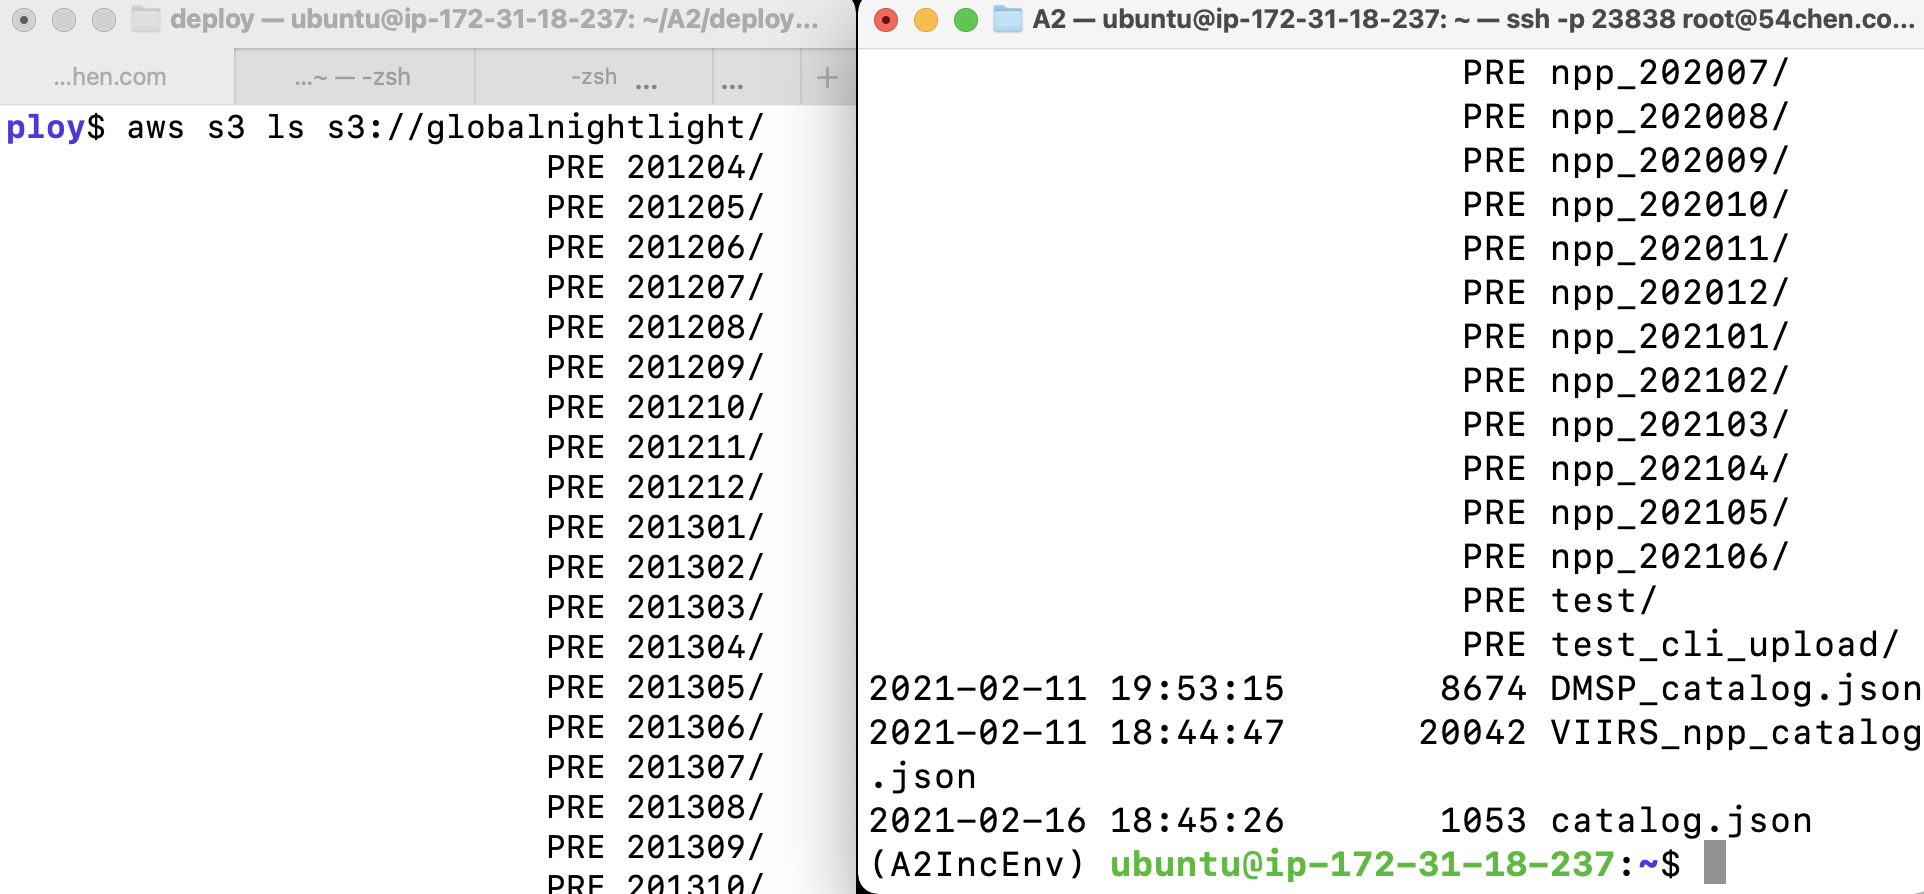
\includegraphics[width=200pt]{images/3.1.png}}
        \caption{World Bank Nighttime Light Data}
        \label{wbs3}
      \end{figure}
    \end{columns}
  \end{frame}
  
\begin{frame}[fragile]{Background: COG}

  \begin{columns}
    \column{0.5\textwidth}
    
    \begin{figure}[htbp]
      \centerline{
\includegraphics[width=200pt]{images/youtube.png}}
      \caption{COG}
      \label{youtube}
    \end{figure}

    \column{0.5\textwidth}
    All imagery is stored in S3 by Cloud Optimized GeoTIFF (COG) \citep{CloudOpt5:online}.
  \end{columns}
\end{frame}

\begin{frame}[fragile]{Background: STAC}

  \begin{columns}
    \column{0.5\textwidth}
    
    \begin{figure}[htbp]
      \centerline{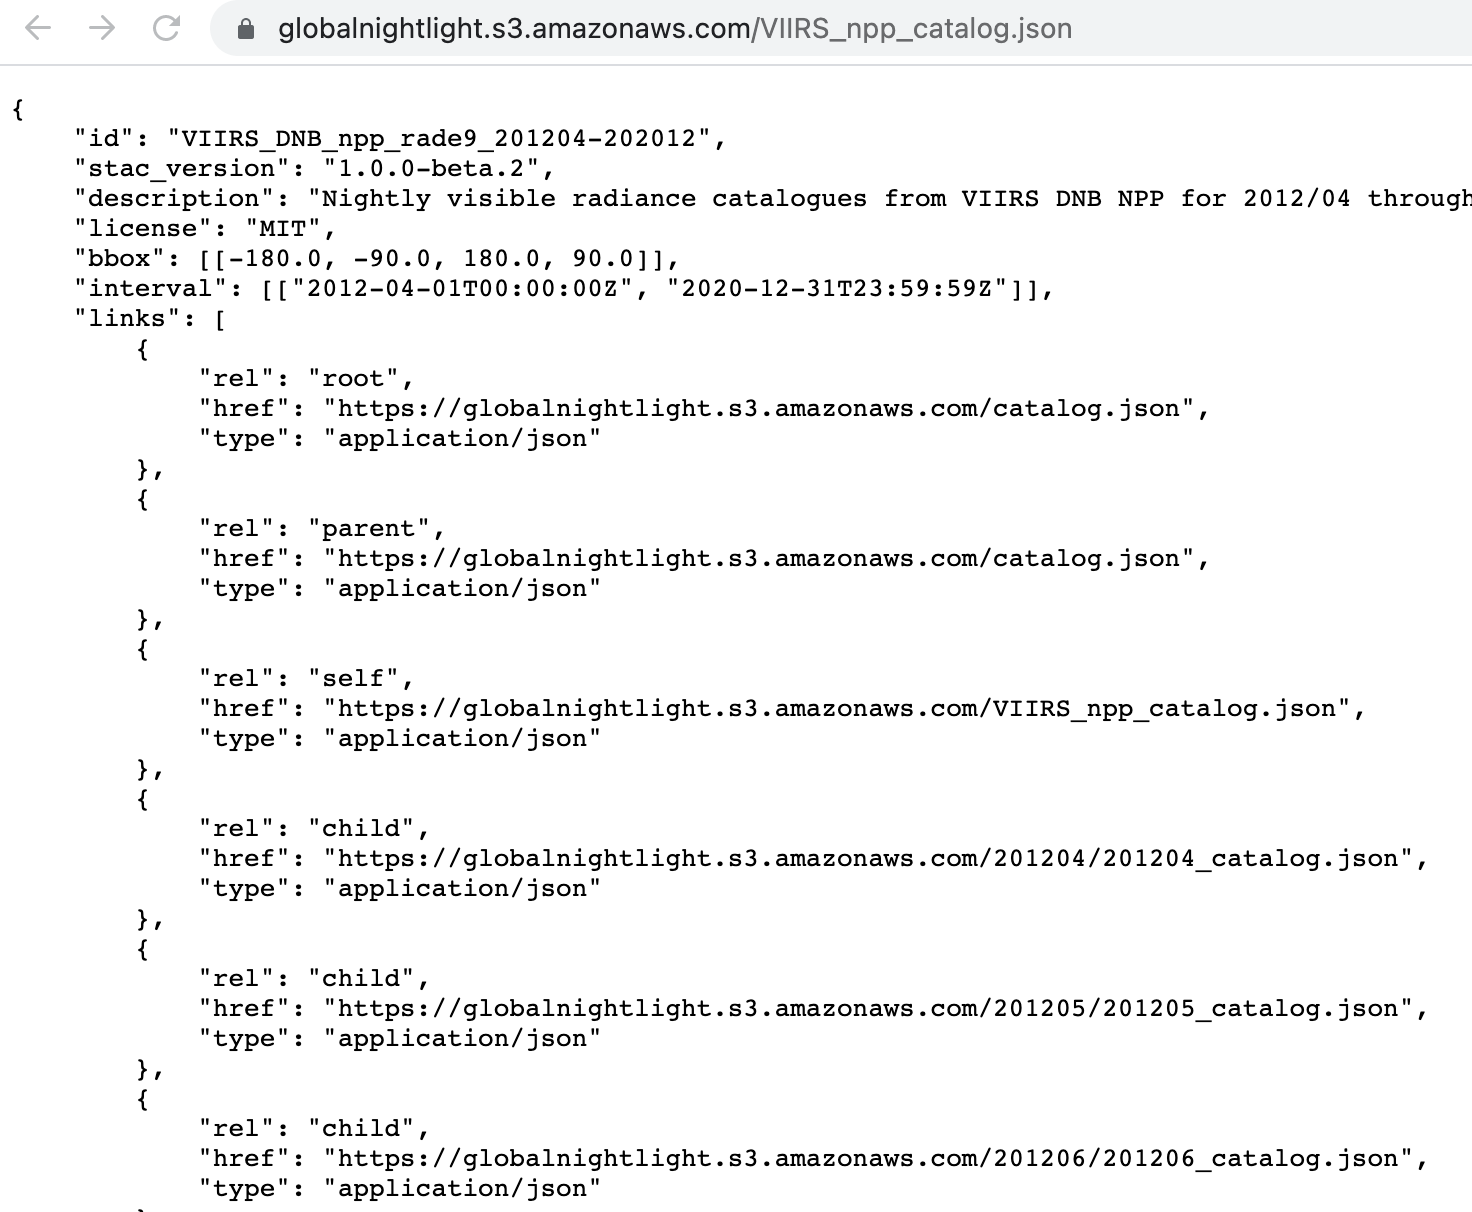
\includegraphics[width=160pt]{images/STAC.png}}
      \caption{STAC of Global ngiht lights}
      \label{STAC}
    \end{figure}

    \column{0.5\textwidth}
    All of the imagery and metadata is organized by Spatial Temporal Asset Catalog (STAC) \citep{SpatioTe90:online}. 
  \end{columns}
\end{frame}

\begin{frame}[fragile]{Background: Objective}

  \begin{columns}
    \column{0.5\textwidth}
    Our objective is to build a demo to show the ngihttime lights status in 3 specific areas.
    \column{0.5\textwidth}
      \begin{figure}[htbp]
        \centerline{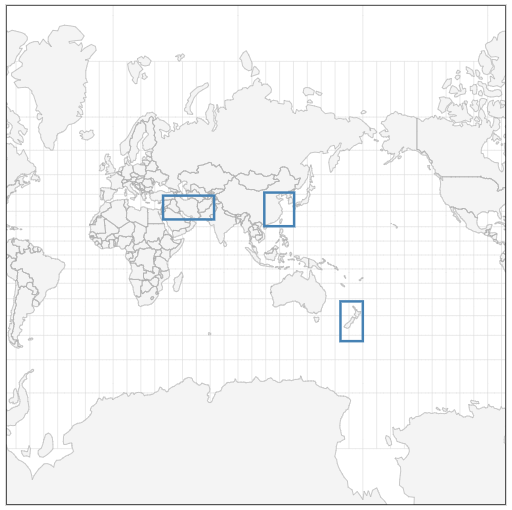
\includegraphics[width=130pt]{images/Worldmap.png}}
        \caption{3 areas we researched}
        \label{areas}
      \end{figure}
  \end{columns}
\end{frame}

\section{Architecture}

\begin{frame}[fragile]{Architecture}
  
  \begin{figure}[htbp]
    \centerline{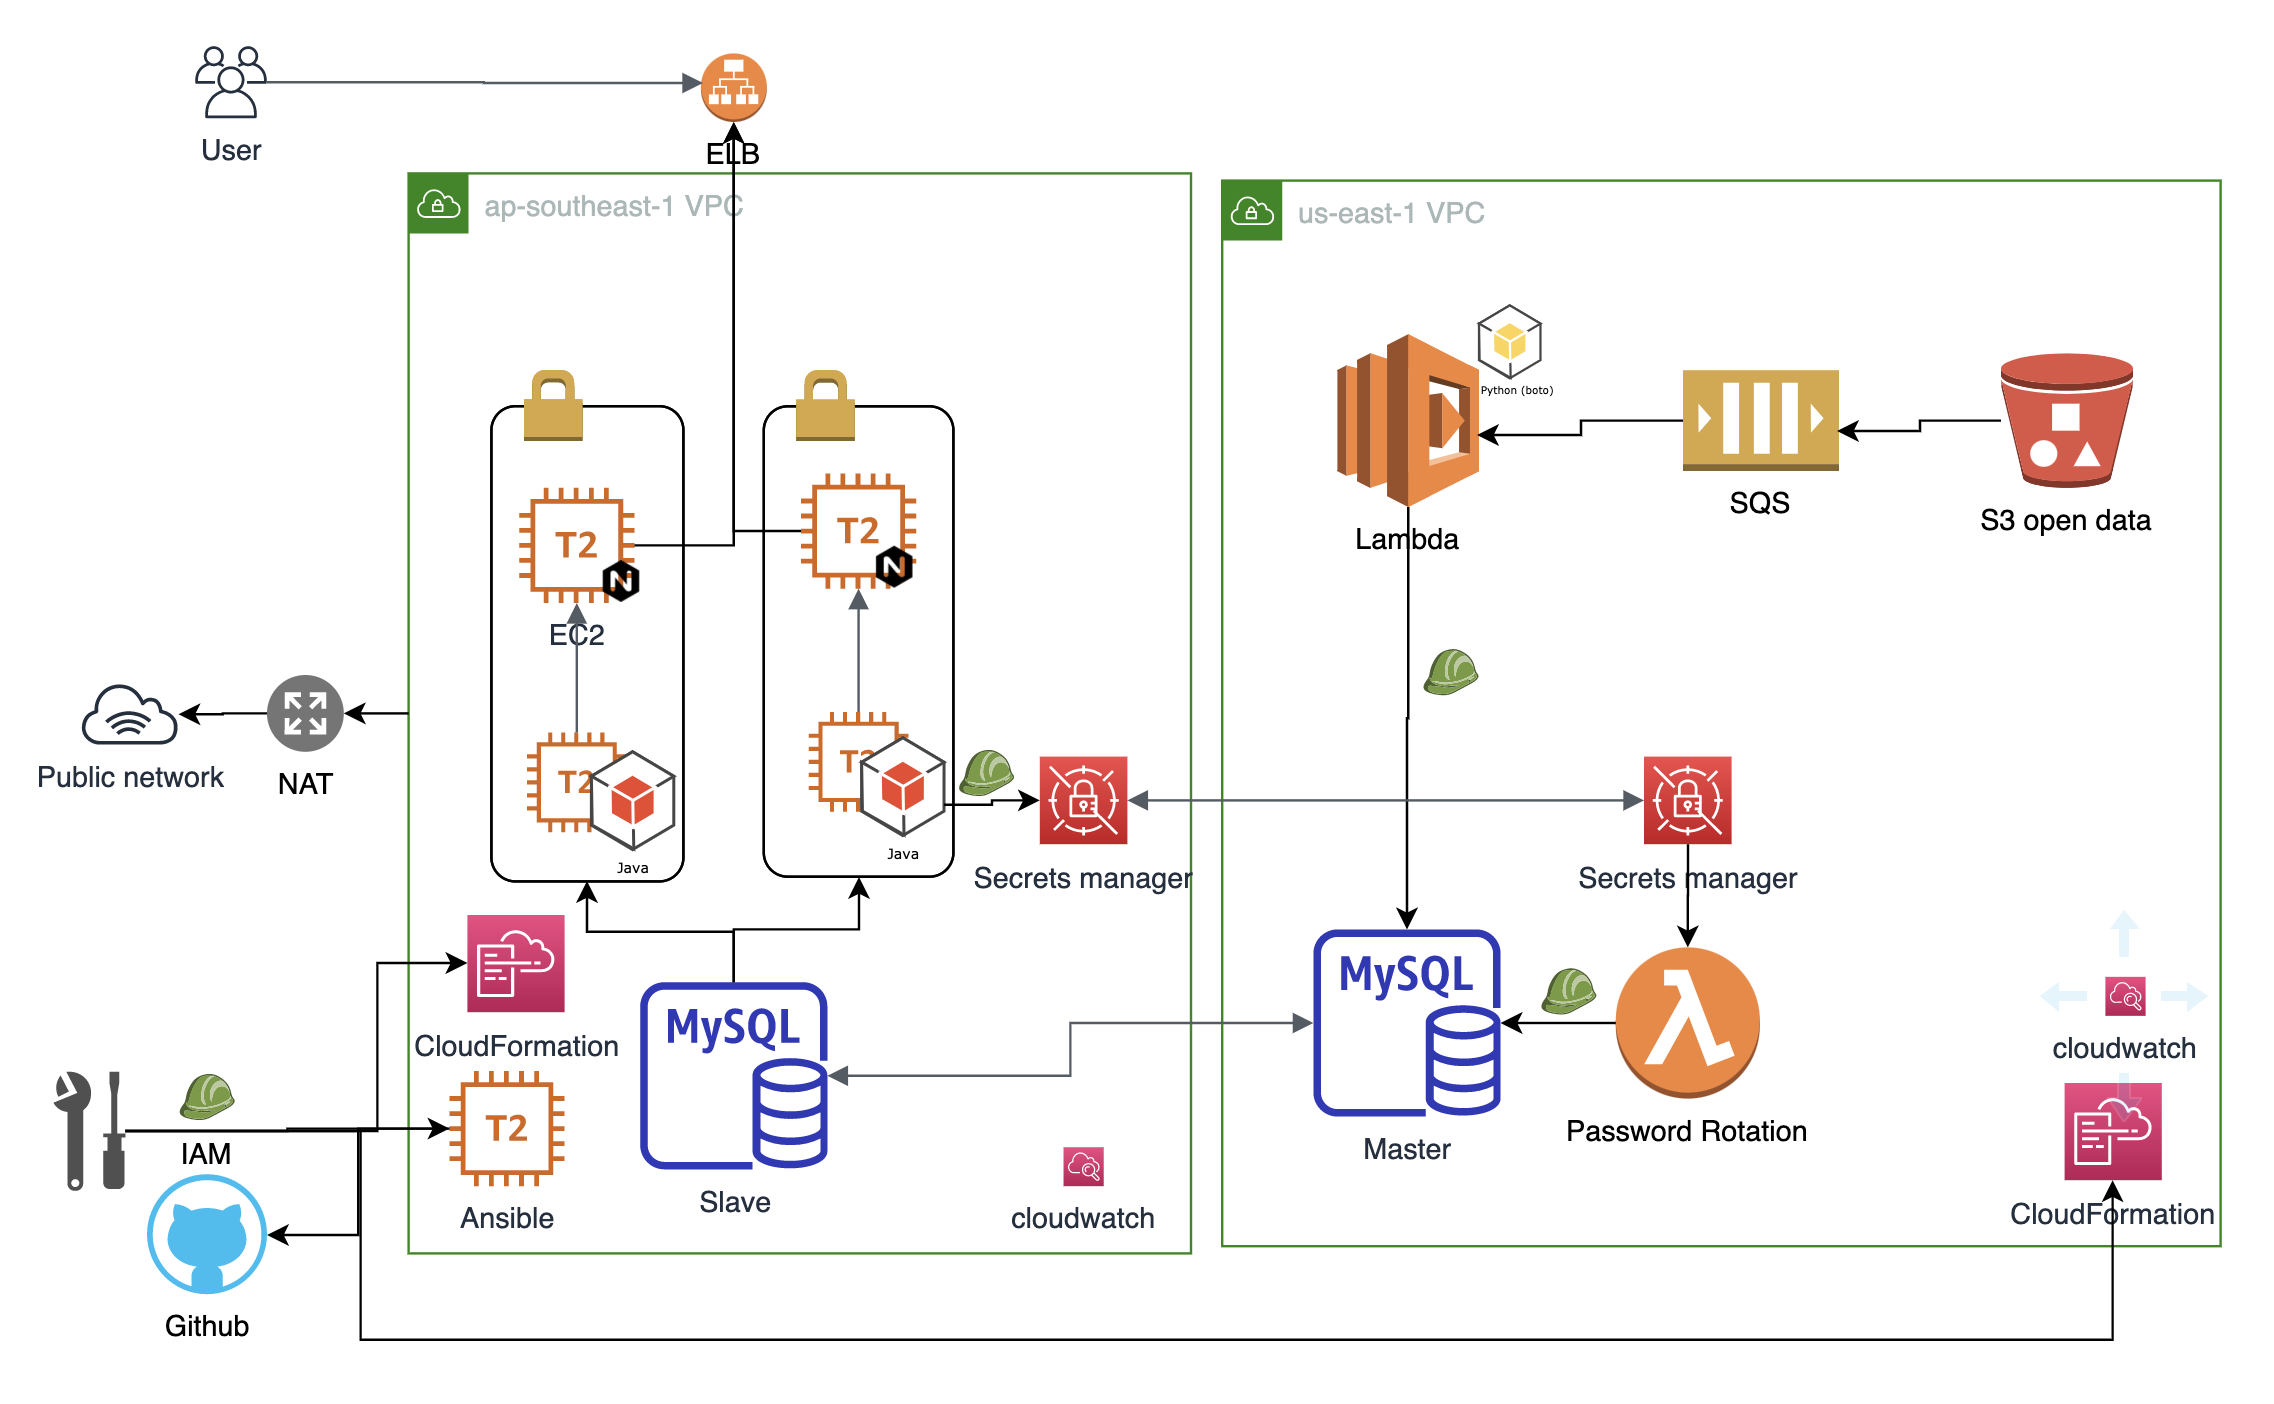
\includegraphics[width=220pt]{images/arch.png}}
    \caption{Architecture}
    \label{fig2}
  \end{figure}

\end{frame}

\begin{frame}[fragile]{Architecture: Backend}

  \begin{columns}
    \column{0.5\textwidth}
      \begin{figure}[htbp]
        \centerline{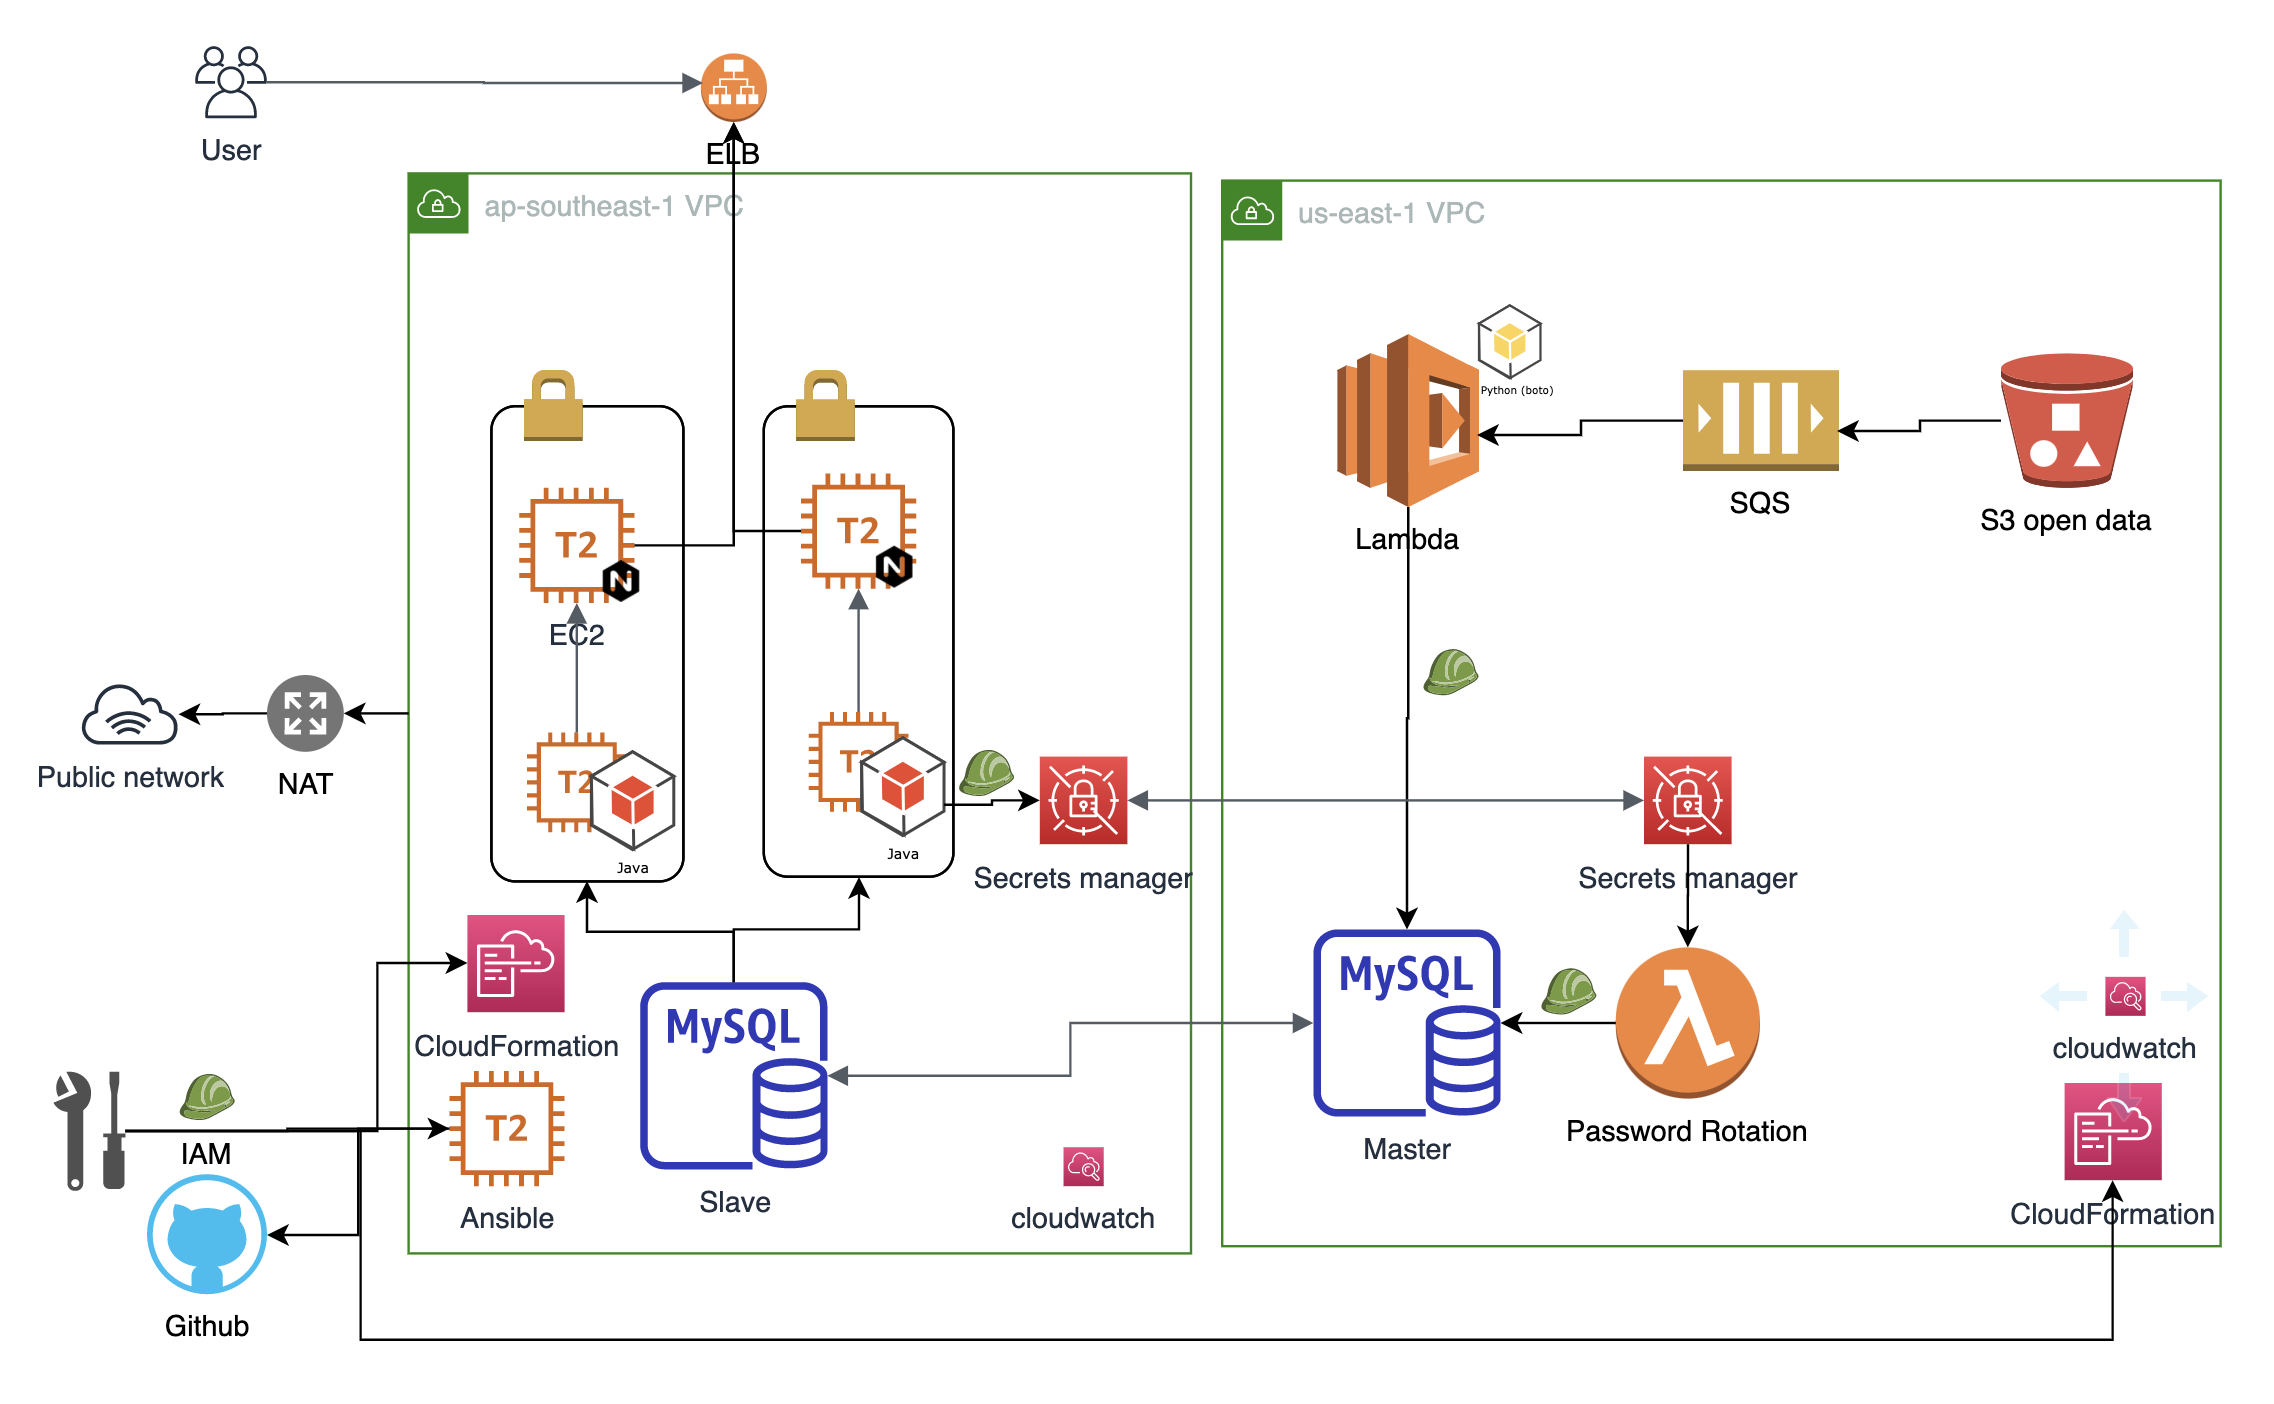
\includegraphics[width=220pt]{images/arch.png}}
        \caption{Architecture}
        \label{arch}
      \end{figure}
    \column{0.5\textwidth}
      \begin{itemize}
        \item EC2: Nginx*2 + Tomcat*2
        \pause
        \item RDS: MySQL
        \pause
        \item Secrets Manager: store the password
        \pause
        \item Lambda: generating passwords \& processing imagery
        \pause
        \item SQS: supporting Lambda fucntions
        \pause
        \item ELB \& NAT: entrance of the demo
        \pause
        \item Others: CloudFormation, CloudWatch, MySQL replica, IAM, S3 etc.
      \end{itemize}
  \end{columns}

\end{frame}

\begin{frame}[fragile]{Architecture: Frontend Technical basis}

	\begin{figure}[htbp]
		\centerline{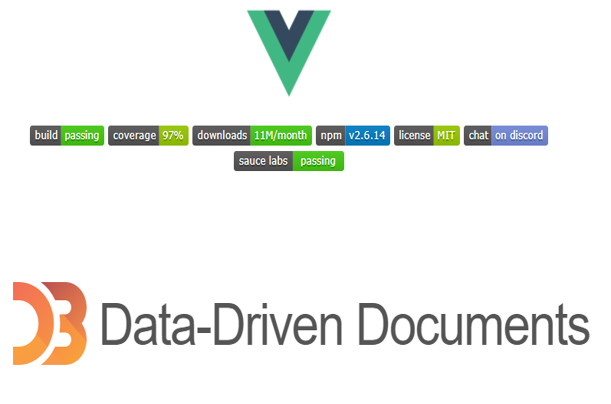
\includegraphics[width=200pt]{images/VueAndD3.png}}
        \caption{Vue.js + D3.js}
    \end{figure}

\end{frame}

\begin{frame}[fragile]{Architecture: Frontend Function}

  \begin{columns}
    \column{0.66\textwidth}
      \begin{figure}[htbp]
        \centerline{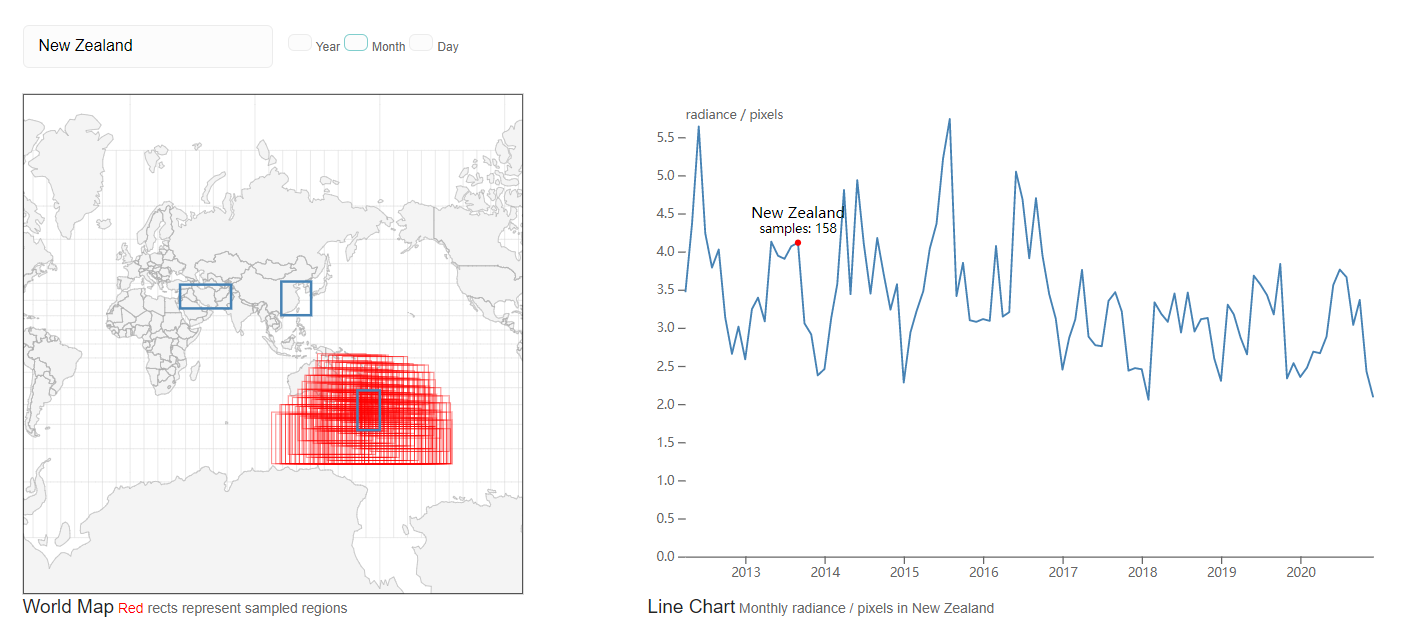
\includegraphics[width=220pt]{images/Interaction_of_visualization.png}}
        \caption{Data visualization}
       \end{figure}

    \column{0.33\textwidth}
      \begin{itemize}
        \item 3rd party login
        \pause
        \item Data visualization
		\pause
		\item (1) Line chart
		\pause
		\item (2) World map
		\pause
		\item (3) Interaction
      \end{itemize}
  \end{columns}

\end{frame}

\section{Security implementation}

\begin{frame}[fragile]{Security implementation: Frontend}

  \begin{columns}
    \column{0.5\textwidth}
	  \begin{itemize}
        \item What Vue Does to Protect You
        \pause
        \item HTML content is automatically escaped.
        \item Attribute bindings are also automatically escaped.
      \end{itemize}

    \column{0.5\textwidth}
      \begin{itemize}
        \item Business perspective
		\pause
        \item No user-provided content
        \pause
        \item No state change
		\pause
		\item httpOnly Cookies
      \end{itemize}
  \end{columns}

\end{frame}

\begin{frame}[fragile]{Security implementation: IAM}

  \begin{columns}
    \column{0.5\textwidth}
      \begin{figure}[htbp]
        \centerline{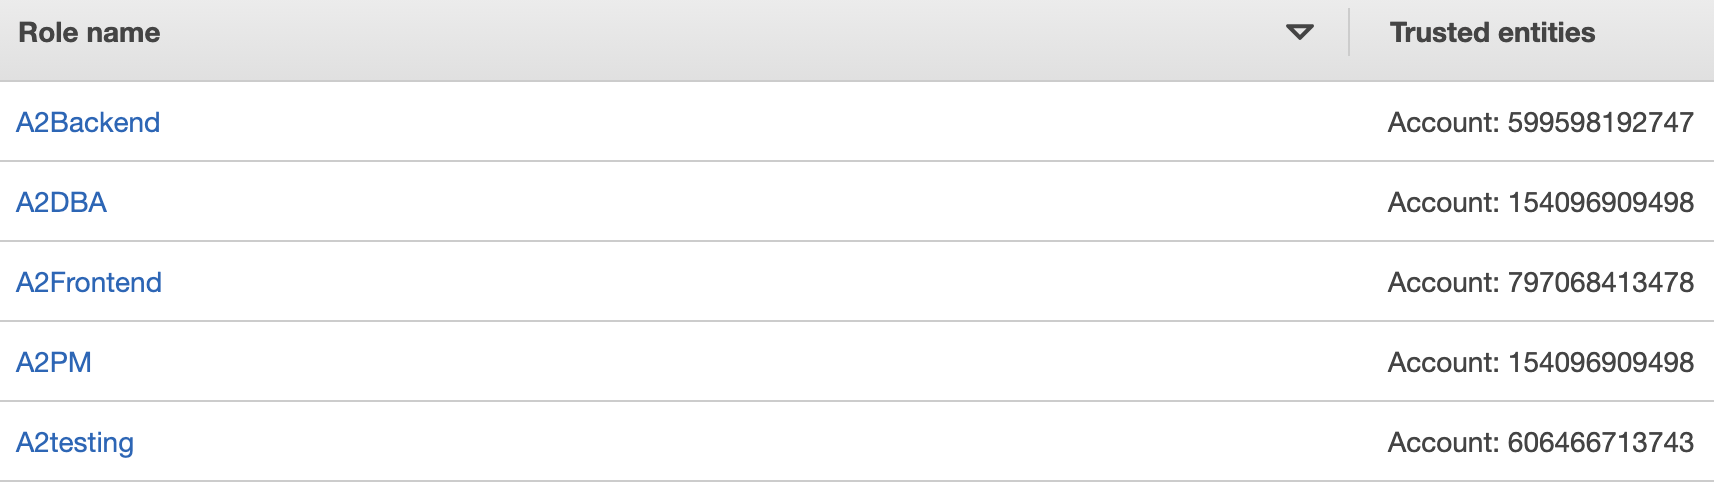
\includegraphics[width=220pt]{images/roles.png}}
        \caption{Roles}
        \label{roles}
      \end{figure}
    \column{0.5\textwidth}
      \begin{itemize}
        \item open the MFA login
        \item divide into Roles: team members \& services
        \item least privileges
        \pause
        \item Users: Github Oauth.
      \end{itemize}
  \end{columns}

\end{frame}


\begin{frame}[fragile]{Security implementation: Network}

  \begin{columns} 
    \column{0.5\textwidth}
      \begin{figure}[htbp]
        
        \centerline{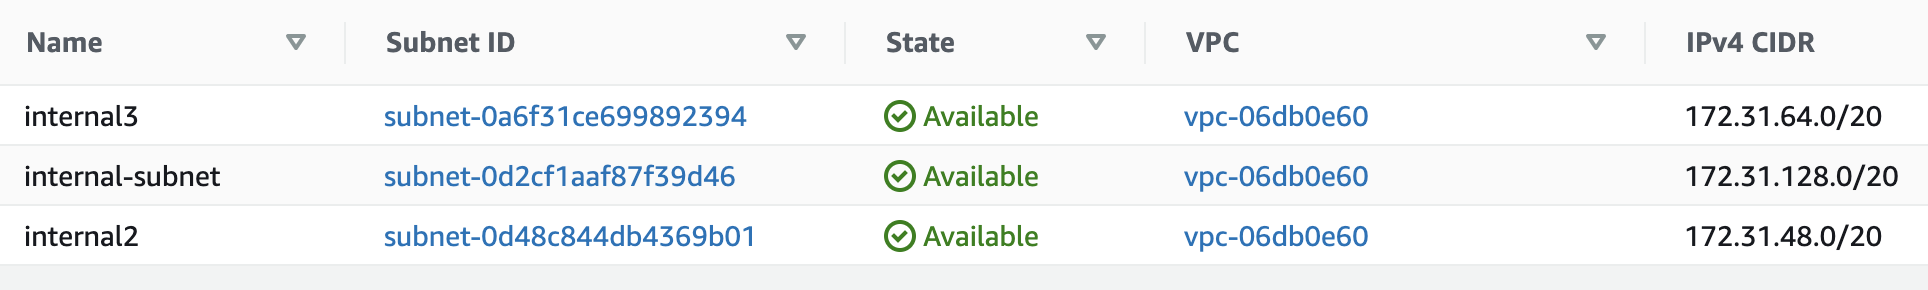
\includegraphics[width=200pt]{images/subnet.png}}
        \caption{Subnet}

        \centerline{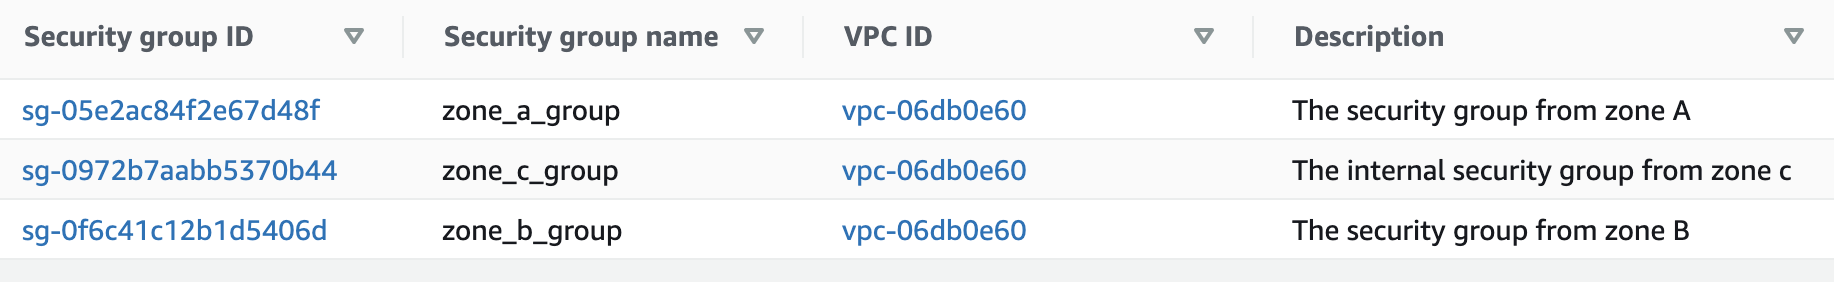
\includegraphics[width=200pt]{images/security.png}}
        \caption{Security groups}

      \end{figure}
    \column{0.5\textwidth}
      \begin{itemize}
        \item isolate public IP instances with others by subnet
        \pause
        \item 3 different subnets used for services in different layers
        \pause
        \item 3 zones are divided into 3 subnets
      \end{itemize}
  \end{columns}

\end{frame}


\begin{frame}[fragile]{Security implementation: Data security}

  \begin{columns}
    \column{0.5\textwidth}
      \begin{figure}[htbp]
        \centerline{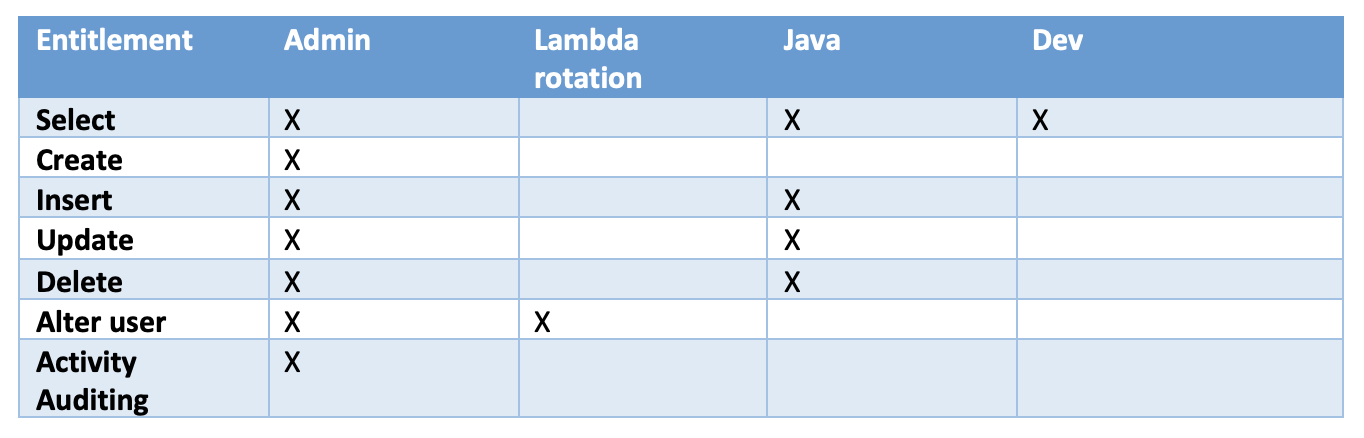
\includegraphics[width=180pt]{images/matrix.png}}
        \caption{Entitlement matrix}
      \end{figure}
    \column{0.5\textwidth}
      \begin{itemize}
        \item Identification \& Category: public original data, imagery data after processing, user data
        \pause
        \item Admin account is the supper administrator
        \pause
        \item Encryption: HTTPS \& RDS KMS \& GitHub Oauth
      \end{itemize}
  \end{columns}

\end{frame}


\begin{frame}[fragile]{Security implementation: Testing}

  \begin{columns}
    \column{0.5\textwidth}
% Picture insert here
      \begin{figure}[htbp]
        \centerline{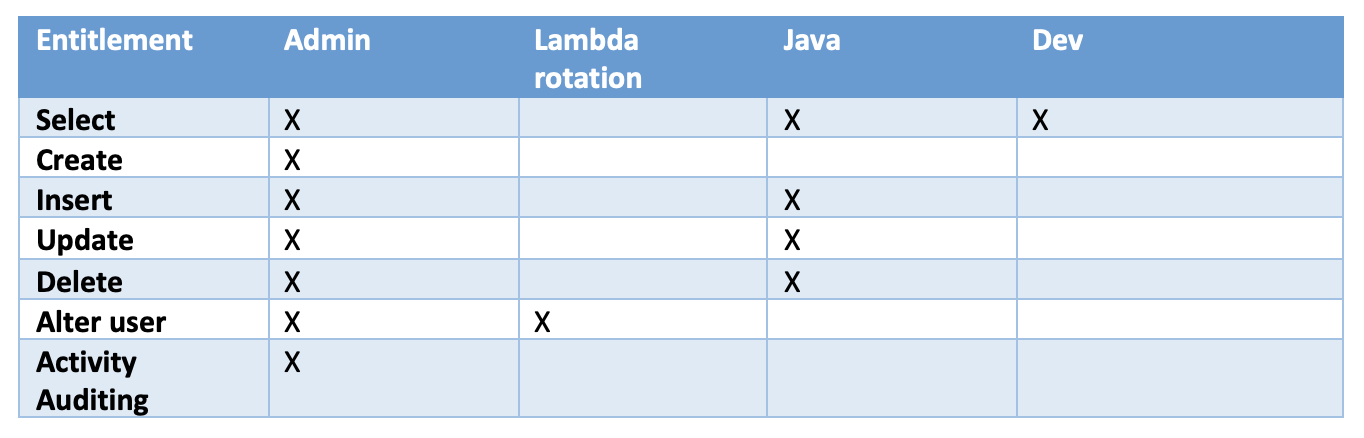
\includegraphics[width=180pt]{images/matrix.png}}
        \caption{Entitlement matrix}
      \end{figure}

    \column{0.5\textwidth}
      \begin{itemize}
% One item one page
        \item Identification \& Category: public original data, imagery data after processing, user data
        \pause
        \item Admin account is the supper administrator
        
      \end{itemize}
  \end{columns}

\end{frame}

\section{Video time}

\section{Reference}

\begin{frame}[allowframebreaks]{Reference}

   \printbibliography[heading=none]
 
\end{frame}

\begin{frame}{}
  \textbf{Thanks}

  \textbf{Q\&A}
\end{frame}

\end{document}
